\chapter{Introdução} \label{chapter:introducao}

Os  avanços nas  tecnologias  de  redes sem  fio  contribuíram para  o
surgimento  da rede  ad hoc  móvel,  do inglês  \textit{Mobile Ad  hoc
  Network} (MANET).  MANET é um tipo de rede autoconfigurável composta
por um conjunto de nós móveis independentes que são conectados uns aos
outros utilizando redes  sem fio.  Cada nó em uma  MANET pode se mover
livremente, logo, é comum que suas conexões se alterem com frequência.
Estes  nós   normalmente  são  dispositivos  tais   como  computadores
pessoais,   pequenos  dispositivos   móveis,   sensores  e   telefones
celulares.

Há diversas pesquisas interessadas em desenvolver projetos de sistemas
de  transporte  inteligentes, visando  uma  melhoria  na segurança  em
estradas  \cite{SINGH2015,tatari:2012}.    Um  dos   mais  importantes
sistemas  de transporte  inteligente é  um tipo  particular de  MANET,
conhecido   como    \textit{Vehicular   Ad   hoc    Network}   (VANET)
\cite{BITAM2013981}. Nas VANETs, o conjunto  de nós da rede é composto
por veículos que se movem de  acordo com padrões restritos baseados em
fatores como  sentido da  via, regulamentações  de trânsito  e tráfego
\cite{PLOL2008390}. Uma  VANET provê  comunicação entre  veículos, que
pode  ser de  duas maneiras  distintas: apenas  entre veículos  (V2V -
\textit{Vehicle to vehicle}) e  entre veículos e infraestruturas fixas
distribuídas ao longo  da estrada como estações  base, também chamados
de RSU (Roadside Unit), (V2I - \textit{Vehicle to Infrastructure}).

Segundo Karim \cite{karim:2008}, a aplicação de VANETs é mais indicada
para  comunicação de  redes veiculares  por possuir  uma sequência  de
vantagens, tais como o baixo  custo de implantação, a possibilidade de
comunicação em locais  onde não existem infraestruturas  fixas e baixa
latência na entrega  de pacotes de dados, quando  comparada com demais
tecnologias           como           redes           3G/4G           e
\textit{infostation}\footnote{\textit{Infostation} é  um tipo  de rede
que oferece grande cobertura geográfica e em alta velocidade, contanto
que  as  aplicações  tenham  tolerância a  atrasos  significativos  na
entrega.}.
 
As aplicações em VANETs são  utilizadas principalmente para auxiliar a
comunicação e coordenação entre condutores de veículos, com o objetivo
de  orientá-los  para  evitar   eventos  como  acidentes  na  estrada,
engarrafamentos,  estradas em  más condições,  assim como  auxiliar no
controle do limite máximo  de velocidade, levar informações detalhadas
sobre acidentes para  as equipes de resgate e  permitir passagem livre
de  veículos de  emergência.   Outra  categoria de  aplicação  é a  de
entretenimento e conforto para passageiros  e motoristas, com acesso à
Internet, chats,  jogos interativos,  reconhecimento de  locais livres
para estacionamento, dados sobre o preço do combustível, entre outros.
Um dos cenários de funcionamento de VANETs, utilizando comunicação V2V
e V2I, é apresentada na Figura \ref{fig:cen-vanet}.

\begin{figure}[!ht]
  \centerline{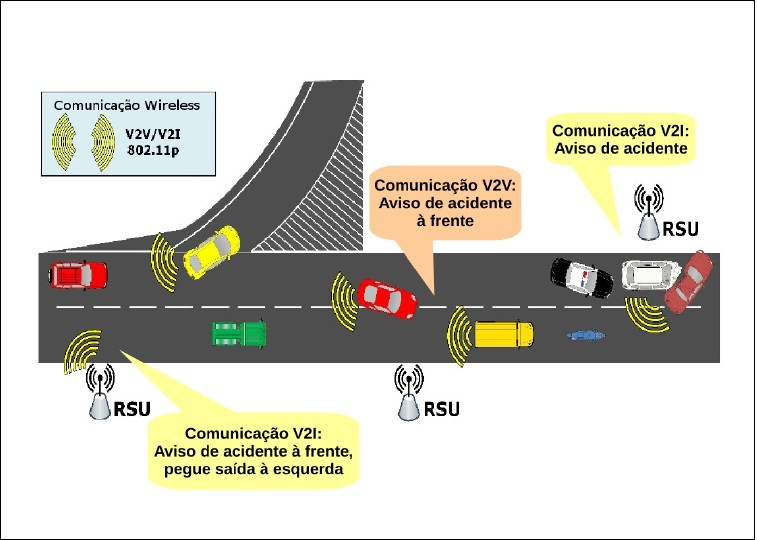
\includegraphics[scale=0.6]{imagens/vanet-comunicacao.jpg}}
  \caption[Shorter figure  caption]{Exemplo de funcionamento de  uma rede VANET.
(Fonte \cite{vehicular})} \label{fig:cen-vanet}
\end{figure}

A  maior diferença  entre  redes MANETs  e VANETs  está  no padrão  de
mobilidade dos nós, pois as VANETs apresentam uma mobilidade mais alta
e  seus  nós  realizam  movimentos pré  definidos  e  limitados  pelas
estradas.   O  principal  desafio  em  VANETs  consiste  em  manter  o
roteamento estável, uma vez que  as redes geradas pelas conexões entre
veículos são  muito dinâmicas  \cite{mustafa:2011}.  Segundo  Taleb et
al. \cite{taleb:2007},  tendo em vista  a alta mobilidade dos  nós, os
protocolos  de  roteamento  desenvolvidos  para  MANETs  precisam  ser
devidamente   adaptados  para   atender  efetivamente   um  roteamento
otimizado em VANETs.

Segundo  Peterson  et  al.    \cite{Peterson:2011},  em  uma  rede  de
comunicação existem  três métodos  fundamentais para a  transmissão de
dados: \textit{unicast},  \textit{broadcast} e  \textit{multicast}.  O
\textit{unicast}  é  a  forma  de  roteamento  onde  a  comunicação  é
realizada de um  para um, isto é, em cada  transmissão realizada um nó
age como origem e outro  como destino.  A abordagem \textit{broadcast}
realiza comunicação de um para todos, ou seja, um nó age como origem e
todos   os  outros   nós  da   rede  serão   destinos.   Por   fim,  o
\textit{multicast} realiza a comunicação de  um nó que age como origem
para  um   subconjunto  de   nós  que   são  destinos.    A  abordagem
\textit{multicast} é  o método  mais eficiente  para a  comunicação em
grupo, reduzindo  o desperdício  de recursos da  rede e  tornando mais
barato e  rápido o custo de  comunicação, uma vez que  as transmissões
para o conjunto  de nós destino são realizadas com  base em um caminho
lógico definido, sem obrigatoriedade  de replicação da informação para
todos os nós  da rede, independente deles estarem  interessados ou não
na mensagem, como acontece no {\em broadcast}. Uma desvantagem do {\em
  unicast} é  que o método gera  uma cópia da informação  para cada um
dos  nós  pelos  quais  o  pacote de  dados  deve  passar.   A  Figura
\ref{fig:metodos-transmissao}   ilustra   as    três   abordagens   de
transmissão.

\begin{figure}[!ht]
\fbox{
\begin{subfigure}{.3\textwidth}
\begin{tikzpicture}[
            - = stealth, % arrow head style
            %shorten > = 0.7pt, % don't touch arrow head to node
            auto,
            node distance = 0.3cm, % distance between nodes
            semithick % line style
        ]

        \tikzstyle{every state}=[
            draw = black,
            thick,
            fill = black,
            minimum size = 3mm
        ]

        \node[state, fill = white, draw = white] (dummy) [at={(-1.7, 0.2)}] {};
        \node[state, fill = gray] (a) [at={(-1.5, -1)}]{};
        \node[state] (b) [at={(0.5, 0)}] {};
        \node[state] (c) [at={(0.5, -2)}] {};
        %\node[state, scale = 0.01] (d) [at={(-0.2, -1)}] {};
        \node[state, fill = gray, draw = gray] (e) [at={(2, -0.5)}] {};
        \node[state] (f) [at={(2, -1.5)}] {};
        \node[state] (g) [at={(2.5, -1)}] {};
        
        \path[-] (a) edge node {} (e);
        %\path[-] (d) edge node {} (e);        
    \end{tikzpicture}
\subcaption{\label{subfig:unicast} Unicast}
\end{subfigure}} \hfill
% Broadcast
\fbox{
\begin{subfigure}{.3\textwidth}
\begin{tikzpicture}[
            - = stealth, % arrow head style
            %shorten > = 0.7pt, % don't touch arrow head to node
            auto,
            node distance = 0.3cm, % distance between nodes
            semithick % line style
        ]

        \tikzstyle{every state}=[
            draw = gray,
            thick,
            fill = gray,
            minimum size = 3mm
        ]
        \node[state, fill = white, draw = white] (dummy) [at={(-1.7, 0.2)}] {};
        \node[state, draw = black] (d) [at={(-1.5, -1)}]{};
        \node[state] (b) [at={(0.5, 0)}] {};
        \node[state] (c) [at={(0.5, -2)}] {};
        %\node[state, scale = 0.01] (d) [at={(-0.2, -1)}] {};
        \node[state] (e) [at={(2, -0.5)}] {};
        \node[state] (f) [at={(2, -1.5)}] {};
        \node[state] (g) [at={(2.5, -1)}] {};
        
        %\path[-] (a) edge node {} (d);
        \path[-] (d) edge node {} (e);
        \path[-] (d) edge node {} (b);
        \path[-] (d) edge node {} (f);
        \path[-] (d) edge node {} (g);
        \path[-] (d) edge node {} (c);
        
    \end{tikzpicture}
\subcaption{\label{subfig:broadcast} Broadcast}
\end{subfigure}} \hfill
% Multicast
\fbox{
\begin{subfigure}{.3\textwidth}
\begin{tikzpicture}[
            - = stealth, % arrow head style
            %shorten > = 0.7pt, % don't touch arrow head to node
            auto,
            node distance = 0.3cm, % distance between nodes
            semithick % line style
        ]

        \tikzstyle{every state}=[
            draw = gray,
            thick,
            fill = gray,
            minimum size = 3mm
        ]
        \node[state, fill = white, draw = white] (dummy) [at={(-1.7, 0.2)}] {};
        \node[state, draw = black] (d) [at={(-1.5, -1)}]{};
        \node[state] (b) [at={(0.5, 0)}] {};
        \node[state, draw = black, fill = black] (c) [at={(0.5, -2)}] {};
        %\node[state, scale = 0.01] (d) [at={(-0.2, -1)}] {};
        \node[state] (e) [at={(2, -0.5)}] {};
        \node[state] (f) [at={(2, -1.5)}] {};
        \node[state, draw = black, fill = black] (g) [at={(2.5, -1)}] {};
        
        %\path[-] (a) edge node {} (d);
        \path[-] (d) edge node {} (b);
        \path[-] (d) edge node {} (c);
        \path[-] (c) edge node {} (f);
        \path[-] (f) edge node {} (e);
        
    \end{tikzpicture}
\subcaption{\label{subfig:multicast} Multicast}
\end{subfigure}} \hfill
\caption{\label{fig:metodos-transmissao} Métodos usuais para transmissão de dados em redes}
\end{figure}

Em VANETs, assim como em outros  tipos de redes, as aplicações possuem
requisitos especiais em relação aos  recursos da rede.  A qualidade de
serviço, do inglês  \gls{qos}, está diretamente relacionada  com o uso
de demandas  de recursos da rede,  uma vez que em  muitas aplicações é
extremamente importante manter  o serviço da rede  com qualidade alta.
Por exemplo, aplicações relacionadas  à segurança, tais como mensagens
de  aviso de  colisão,  acidentes  ou más  condições  da estrada,  são
sensíveis ao atraso  na entrega das mensagens, bem  como aplicações de
multimídia  são  sensíveis à  largura  de  banda. Dentre  as  métricas
existentes, vale ressaltar algumas que são de extrema importância para
VANETs: atraso fim a fim (\textit{end-to-end delay}), \textit{jitter},
ou seja, variação  no atraso entre as mensagens para  o mesmo destino,
variação do  atraso fim  a fim entre  diferentes destinos,  largura de
banda (\textit{bandwidth}), quantidade de saltos da mensagem, ou seja,
a quantidade de nós pelos quais o  pacote passa até o destino final, e
estimativa de duração da conexão  entre veículos. Neste trabalho serão
consideradas as quatro primeiras  métricas citadas, explicadas em mais
detalhes a seguir.

Entende-se {\delay}  fim a fim como  o tempo gasto para  que um pacote
seja enviado da origem até o  destino.  O tempo total consiste na soma
dos atrasos do processamento nos nós  da rede e o atraso da propagação
ao longo  do meio de transmissão.   O \textit{jitter} é uma  medida da
variação do atraso na entrega entre sucessivos pacotes de dados em uma
conexão.  Para exemplificar, se um pacote enviado de uma origem até um
destino tem atraso  de 15 ms e  o envio de outro pacote  entre a mesma
origem  e destino  tem atraso  de 17  ms, isso  significa, de  maneira
simplificada, que o  {\jitter} dessa conexão é igual a  2 ms.  Segundo
Biradar e  Manvi \cite{biradar:2012},  é possível  reduzir o  valor do
{\jitter}  com  a  utilização de  \textit{buffers},  entretanto,  isso
aumenta consideravelmente a quantidade  de memória necessária, fazendo
com que seja preferível ter  o \textit{jitter} controlado pela própria
rede.

A variação  do {\delay}  entre os diferentes  destinos pode  ser definida
como a  diferença entre o atraso  do caminho que conecta  a origem com
qualquer  par de  destinos.  Limitar  essa variação  é essencial  para
sincronização  entre os  vários  receptores, garantindo  que não  haja
diferença de muitos  pacotes de uma mesma mensagem para  os vários nós
destinatários durante o tempo de vida de uma sessão \textit{multicast}
\cite{rouskas:1997}. Por  exemplo, assumindo um limite  de variação de
atraso entre diferentes destinos como 3 ms, se um pacote leva um tempo
de 17  ms para  ir da origem  para um destino,  um outro  destino deve
receber o  mesmo pacote com  o atraso no  intervalo de $[14,  20]$ ms.
Por fim, a largura de banda é a medida de capacidade de transmissão de
um determinado meio, conexão ou rede, determinando a velocidade máxima
em que os dados podem ser transmitidos no enlace.

De maneira mais informal, o problema de roteamento \textit{multicast},
do inglês \gls{mrp}, pode ser descrito  como um problema onde dados os
custos de transmissão de  mensagens entre veículos, busca-se minimizar
os  gastos  para  transferir  mensagens nó  raiz  até  um  determinado
subconjunto de  nós terminais.  Essa transmissão  pode utilizar outros
nós  da rede,  mas  não  precisa passar  por  todos eles.   Considerar
restrições de Qualidade  de Serviço, do inglês  \gls{qos}, trata-se de
garantir que  os caminhos percorridos  para realizar a  transmissão da
raiz para cada nó terminal  obedeçam às restrições de \gls{qos}. Essas
considerações resultam no \gls{mrp-qos}.

Uma propriedade essencial para garantir  que uma instância do \gls{mrp-qos} seja
viável é que exista pelo menos uma solução na qual todos os nós terminais possam
ser  atendidos.  Tipicamente  em  VANETs os  veículos  podem  ocasionalmente  se
desconectarem da  rede em  virtude de  suas elevadas  mobilidades, ou  seja, nem
sempre  é  possível garantir  que  todos  os  veículos  serão atendidos  a  todo
instante. Sendo assim, este trabalho propões uma nova variante do \gls{mrp-qos},
denominada  Máximo Atendimento  em  \gls{mrp} com  restrições  de \gls{qos},  do
inglês \gls{pma}, onde  nem todos os nós terminais da  rede podem ser atendidos.
Se o  caminho gerado  da raiz até  um terminal respeita  todas as  restrições de
\gls{qos}, esse terminal atendido, caso contrário,  o terminal não é atendido. O
objetivo do \gls{pma} é maximizar o serviço, i.e., atender o maior número de nós
terminais de acordo com as métricas de \gls{qos} impostas pela rede.

A Figura \ref{fig:ex1} apresenta um  exemplo do processo que constitui
a resolução  de uma  instância do  \gls{pma}. A  Figura \ref{subfig:a}
representa  o  grafo inicial,  tal  que  os nós  retangulares  (azuis)
representam  o conjunto  de veículos  terminais (destinos),  o nó  com
círculo  duplo (vermelho)  é o  nó raiz,  enquanto os  demais nós  são
opcionais.   Todas as  conexões  (links) tem  arcos bidirecionais,  ou
seja,  se  por exemplo  os  nós  1 e  4  estão  conectados é  possível
encaminhar mensagens na direção $(1, 4)$ e também $(4, 1)$.  Cada arco
contém 3 métricas associadas,  $\lambda$ ({\delay}), $\xi$ ({\jitter})
e  $\omega$ (largura  de  banda), uma  quarta  métrica utilizada  pelo
\gls{pma} é a de variação de  {\delay s} entre terminais.  No entanto,
ela não se aplica aos arcos individualmente  e sim a todos os pares de
caminhos   utilizados   para   atender   os   terminais.    A   Figura
\ref{subfig:b} apresenta uma solução  do \gls{pma}, onde foram gerados
caminhos, representados  pelos arcos ressaltados (azuis),  que atingem
todos  os  terminais. Nesse  caso  os  terminais com  retângulo  duplo
representam  veículos   atendidos  e   o  retângulo  simples   os  não
atendidos.  Nesse  exemplo,  dos  quatro terminais,  apenas  três  são
atendidos.

\begin{figure}[!ht]
\begin{subfigure}{.5\textwidth}
\begin{tikzpicture}[
            > = stealth, % arrow head style
            shorten > = 0.8pt, % don't touch arrow head to node
            auto,
            node distance = 1.5cm, % distance between nodes
            semithick % line style
        ]

        \tikzstyle{every state}=[
            draw = black,
            thick,
            fill = white,
            minimum size = 8mm
        ]

        \node[state, double, draw=red] (a) [at={(-1.5, -1)}]{$1$};
        \node[state] (b) [at={(2,1)}] {$2$};
        \node[state, rectangle, draw=blue] (c) [at={(4.5,1)}] {$3$};
        \node[state] (d) [at={(0.5, 0.5)}] {$4$};
        \node[state, rectangle, draw=blue] (e) [at={(3,-0.5)}] {$5$};
        \node[state] (f) [at={(2,-2.5)}] {$6$};
        \node[state] (g) [at={(4,-2.5)}] {$7$};
        %\node[state] (h) [at={(3,-2.5)}] {$6$};
        \node[state, rectangle, draw=blue] (i) [at={(0.5,-2.5)}] {$8$};
        \node[state] (j) [at={(5,-0.5)}] {$9$};
        \node[state, rectangle, draw=blue] (k) [at={(5.5,-2.5)}] {$10$};
        
        \path[->] (a) edge node {} (d); 
        \path[->] (d) edge node {} (a); 
        \path[->] (i) edge node {} (a);
        \path[->] (a) edge node {} (i);
        \path[->] (a) edge node {} (e);
        \path[->] (e) edge node {} (a);
        \path[->] (b) edge node {} (d);
        \path[->] (b) edge node {} (e);
        \path[->] (b) edge node {($\lambda$,$\xi$,$\omega$)} (c);
        \path[->] (c) edge node {} (e);
        \path[->] (e) edge node {} (f);
        \path[->] (d) edge node {} (i);
        \path[->] (d) edge node {} (e);
        \path[->] (d) edge node {} (f);
        \path[->] (e) edge node {} (g);
        \path[->] (f) edge node {} (j);
        \path[->] (c) edge node {} (j);
        \path[->] (i) edge node {} (f);
        \path[->] (i) edge node {} (b);
        \path[->] (j) edge node {} (k);
        \path[->] (j) edge node {} (g);
        \path[->] (d) edge node {} (b);
        \path[->] (e) edge node {} (b);
        \path[->] (c) edge node {} (b);
        \path[->] (e) edge node {} (c);
        \path[->] (f) edge node {} (e);
        \path[->] (f) edge node {} (g);
        \path[->] (g) edge node {} (f);
        \path[->] (i) edge node {} (d);
        \path[->] (e) edge node {} (d);
        \path[->] (f) edge node {} (d);
        \path[->] (g) edge node {} (e);
        \path[->] (j) edge node {} (f);
        \path[->] (j) edge node {} (c);
        \path[->] (f) edge node {} (i);
        \path[->] (b) edge node {} (i);
        \path[->] (k) edge node {} (j);
        \path[->] (g) edge node {} (j);
        
    \end{tikzpicture}
\subcaption{\label{subfig:a} Grafo com raiz e terminais}
\end{subfigure}
% Segunda figura
\begin{subfigure}{.5\textwidth}
\begin{tikzpicture}[
            > = stealth, % arrow head style
            shorten > = 0.8pt, % don't touch arrow head to node
            auto,
            node distance = 1.5cm, % distance between nodes
            semithick % line style
        ]

        \tikzstyle{every state}=[
            draw = black,
            thick,
            fill = white,
            minimum size = 8mm
        ]

        \node[state, double, draw=red] (a) [at={(-1.5, -1)}]{$1$};
        \node[state] (b) [at={(2,1)}] {$2$};
        \node[state, double, rectangle, draw=blue] (c) [at={(4.5,1)}] {$3$};
        \node[state] (d) [at={(0.5, 0.5)}] {$4$};
        \node[state, double, rectangle, draw=blue] (e) [at={(3,-0.5)}] {$5$};
        \node[state] (f) [at={(2,-2.5)}] {$6$};
        \node[state] (g) [at={(4,-2.5)}] {$7$};
        %\node[state] (h) [at={(3,-2.5)}] {$6$};
        \node[state, double, rectangle, draw=blue] (i) [at={(0.5,-2.5)}] {$8$};
        \node[state] (j) [at={(5,-0.5)}] {$9$};
        \node[state, rectangle, draw=blue] (k) [at={(5.5,-2.5)}] {$10$};
        
        \path[->, draw = gray, opacity = 0.3] (a) edge node {} (d); 
        \path[->, draw = gray, opacity = 0.3] (d) edge node {} (a); 
        \path[->, draw = gray, opacity = 0.3] (i) edge node {} (a);
        \path[->, draw = blue] (a) edge node {} (i);
        \path[->, draw = blue] (a) edge node {} (e);
        \path[->, draw = gray, opacity = 0.3] (e) edge node {} (a);
        \path[->, draw = gray, opacity = 0.3] (b) edge node {} (d);
        \path[->, draw = gray, opacity = 0.3] (b) edge node {} (e);
        \path[->, draw = gray, opacity = 0.3] (b) edge node {} (c);
        \path[->, draw = gray, opacity = 0.3] (c) edge node {} (e);
        \path[->, draw = gray, opacity = 0.3] (e) edge node {} (f);
        \path[->, draw = gray, opacity = 0.3] (d) edge node {} (i);
        \path[->, draw = gray, opacity = 0.3] (d) edge node {} (e);
        \path[->, draw = gray, opacity = 0.3] (d) edge node {} (f);
        \path[->, draw = blue] (e) edge node {} (g);
        \path[->, draw = gray, opacity = 0.3] (f) edge node {} (j);
        \path[->, draw = gray, opacity = 0.3] (c) edge node {} (j);
        \path[->, draw = gray, opacity = 0.3] (i) edge node {} (f);
        \path[->, draw = gray, opacity = 0.3] (i) edge node {} (b);
        \path[->, draw = blue] (j) edge node {} (k);
        \path[->, draw = gray, opacity = 0.3] (j) edge node {} (g);
        \path[->, draw = gray, opacity = 0.3] (d) edge node {} (b);
        \path[->, draw = gray, opacity = 0.3] (e) edge node {} (b);
        \path[->, draw = gray, opacity = 0.3] (c) edge node {} (b);
        \path[->, draw = blue] (e) edge node {} (c);
        \path[->, draw = gray, opacity = 0.3] (f) edge node {} (e);
        \path[->, draw = gray, opacity = 0.3] (f) edge node {} (g);
        \path[->, draw = gray, opacity = 0.3] (g) edge node {} (f);
        \path[->, draw = gray, opacity = 0.3] (i) edge node {} (d);
        \path[->, draw = gray, opacity = 0.3] (e) edge node {} (d);
        \path[->, draw = gray, opacity = 0.3] (f) edge node {} (d);
        \path[->, draw = gray, opacity = 0.3] (g) edge node {} (e);
        \path[->, draw = gray, opacity = 0.3] (j) edge node {} (f);
        \path[->, draw = gray, opacity = 0.3] (j) edge node {} (c);
        \path[->, draw = gray, opacity = 0.3] (f) edge node {} (i);
        \path[->, draw = gray, opacity = 0.3] (b) edge node {} (i);
        \path[->, draw = gray, opacity = 0.3] (k) edge node {} (j);
        \path[->, draw = blue] (g) edge node {} (j);
    \end{tikzpicture}
\subcaption{\label{subfig:b} Caminho da mensagem}
\end{subfigure}
\caption{\label{fig:ex1} Exemplo de Instância do MS-MRP-QoS}
\end{figure}

Neste trabalho investigamos o \gls{pma} visando encontrar metodologias
eficazes para  resolvê-lo.  Para alcançar esse  objetivo, inicialmente
resolvemos  o  \gls{pma}  de   maneira  exata  utilizando  \gls{plim}.
Desenvolvemos  um  conjunto  de quatro  relaxações  lagrangianas  para
obtenção de limitantes inferiores e  superiores com base na dualização
de  restrições complicadoras.   Por fim,  foram desenvolvidos  métodos
heurísticos para obter  soluções sem garantia de  otimalidade, mas com
um  baixo uso  de recursos  computacionais.  Uma  heurística de  busca
local  em  arborescências  foi  aplicada   com  objetivo  de  gerar  e
aperfeiçoar soluções viáveis em conjunto  com a solução das relaxações
lagrangianas.   Também foram  propostos três  Algoritmos Genéticos  de
Chaves Aleatórias Viciadas, do  inglês \gls{brkga}, contendo variações
no decodificador, no  cálculo da função objetivo e  no procedimento de
geração das chaves aleatórias.  Por fim, as instâncias utilizadas para
os experimentos foram  geradas utilizando simuladores de  tráfego e de
rede.

Esta  dissertação  está  organizada  em seis  capítulos.   O  Capítulo
\eqref{chp:preliminares}  introduz notações  e definições  necessárias
para o  entendimento dos demais  capítulos, incluindo a  descrição dos
modelos de \gls{pli} e \gls{plim}, e as principais técnicas utilizadas
neste   trabalho   são  descritas   de   modo   geral.   No   Capítulo
\ref{chp:trab-relacionados},  as principais  publicações presentes  na
literatura  para  problemas  de  otimização em  redes  veiculares  são
apresentadas,   com  foco   nos  resultados   obtidos.   No   Capítulo
\ref{chapter:metodologia}, são  discutidas as  metodologias utilizadas
no  desenvolvimento deste  trabalho.  A  descrição dos  experimentos e
resultados  computacionais é  feita no  Capítulo \ref{chp:resultados}.
Por   fim,   o   Capítulo   \ref{chp:consideracoes-finais}   traz   as
considerações finais do trabalho, seguido das referências.

